\newpage
\section{Coupling growing rootsystems to numerical models} \label{sec:growing}

After coupling a static root system to a soil model, it is straight forward to couple a growing root system. All there is to do is to update the geometry and the mapping between the grids in every time step. All the work is done by MappedRootSystem.

    
\subsection{Mapping of growing roots and underlying soil} 

In the following we show how the mappings between root system grid and soil grids are updated (see Section \ref{ss:mapping} for the static case). For demonstration we create an animation, where we can see the growth and the dynamic mapping. 

\lstinputlisting[firstline=1, language=Python, caption=Example 7a]{../../examples/python/example7a_mapping.py}

\begin{itemize}
\item[8-12] Parameters we might want to modify. 
\item[15-18] Initializes the model.
\item[21-27] Defines a coarse soil grid. If we do not use periodicity we set the domain as confining geometry to the root growth. L27 sets the underlying soil grid.
\item[29-31] Initializes the simulation with an initial simulation run for rs\_age.
\item[33-39] Initializes an VTK animation using the class vp.AnimateRoots, which is work in progress. 
\item[41-59] The simulation loop: L43 performs the simulation, and updates the mappers (no additional steps are needed, everything is updated by pb.MappedRootSystem). L46-52 determines the cell index for each segment for visualization. L54,L L55 makes a SegmentAnalyser object and adds the soil cell indices. L57-L58 updates the animation figure. This is convenient for debugging, and the object vp.AnimateRoots will create an ogg vorbis movie file (which is small and high quality), but for bigger root systems this will be very slow, since a SegmentAnalyser object is created and plotted for each frame (see Section \ref{ssec:animation} for a faster method).
\end{itemize}

\subsection{Coupling a dynamic root system to DuMux with soil feedback} \label{sec:dumux_dyn_coupling}

We modify Example \ref{sec:dumux_coupling}. Using the class MappedRootSystem (as before) it is sufficient to call MappedRootSystem::simulate() to implement real root growth, i.e. to add rs.simulate(dt) in L80. The modified segments and the mapping of new segments is automatically managed (see example7b\_coupling.py). Figure \ref{fig:example7c} shows the root actual uptake over time, with a slightly altered shape compared to \ref{fig:example6c}. Note that the jumps in actual uptake are due to emerging root segments.

In this example soil state does not affect root system growth in any way. We need to add the processes we are interested in (see Section \ref{sec:tropism} and \ref{sec:functional}). For demonstration how to do that, we demonstrate the implementation steps using hydrotropim. Note that the other interactions from Section \ref{sec:functional} could be implemented in the same way. 

In order to use hydrotropism, we need to define a SoilLookUp that accesses the dynamic soil data. We present two approaches: the first uses nearest neighbour interpolation, which is fast but a coarse approximation. The second uses linear interpolation which is more exact, but slower. 

\lstinputlisting[firstline=1, language=Python, caption=Example 7c]{../../examples/python/example7c_feedback.py}

We only describe the changes to Section \label{sec:dumux_coupling}:

\begin{itemize}
\item[18-25] We first create a class for nearest neighbour interpolation that extends pb.SoilLookUp. L22 stores a reference to the DuMux soil model. For specialisation of pb.SoilLookUp we need to overwrite the getValue function (L24-25). First we retrieve the cell index by calling $pick$. And, then we return the solution at this cell (in Pascal). Note that the solution is the same for each point within a cell. 
\item[28-41] Secondly, we want to use linear interpolation, which is slower, but more exact. The constructor stores a reference to the soil model (L30-34) the coordinates of the degrees of freedom (i.e. where the points where numerical solution is defined) and calls update(), which fetches the current model solution. Update will be called in after each solving step in the simulation loop. L39-L41 performs the linear interpolation. This is rather slow because the method assumes an unstructured grid, and is not optimized for a structured rectangular grid. 
\item[94-100] We set tropism to hydrotropism (L98) and modify the tropism parameters (L99,100)
\item[102,103] We set the soil, using nearest neighbour or linear interpolation.
\item[120,121] If we use linear interpolation we need to call update to copy the current solution. 
\item[122] Root system simulation, updates geometry and mappers.

\end{itemize}

Figure \ref{fig:example7c} shows that hydrotropism will lead to increased cumulative uptake, because the roots are more evenly distributed. Note that there is a big variation in the results, and for a more profound analysis we would have to make many simulation runs. 

\begin{figure}
\begin{subfigure}[c]{1\textwidth}
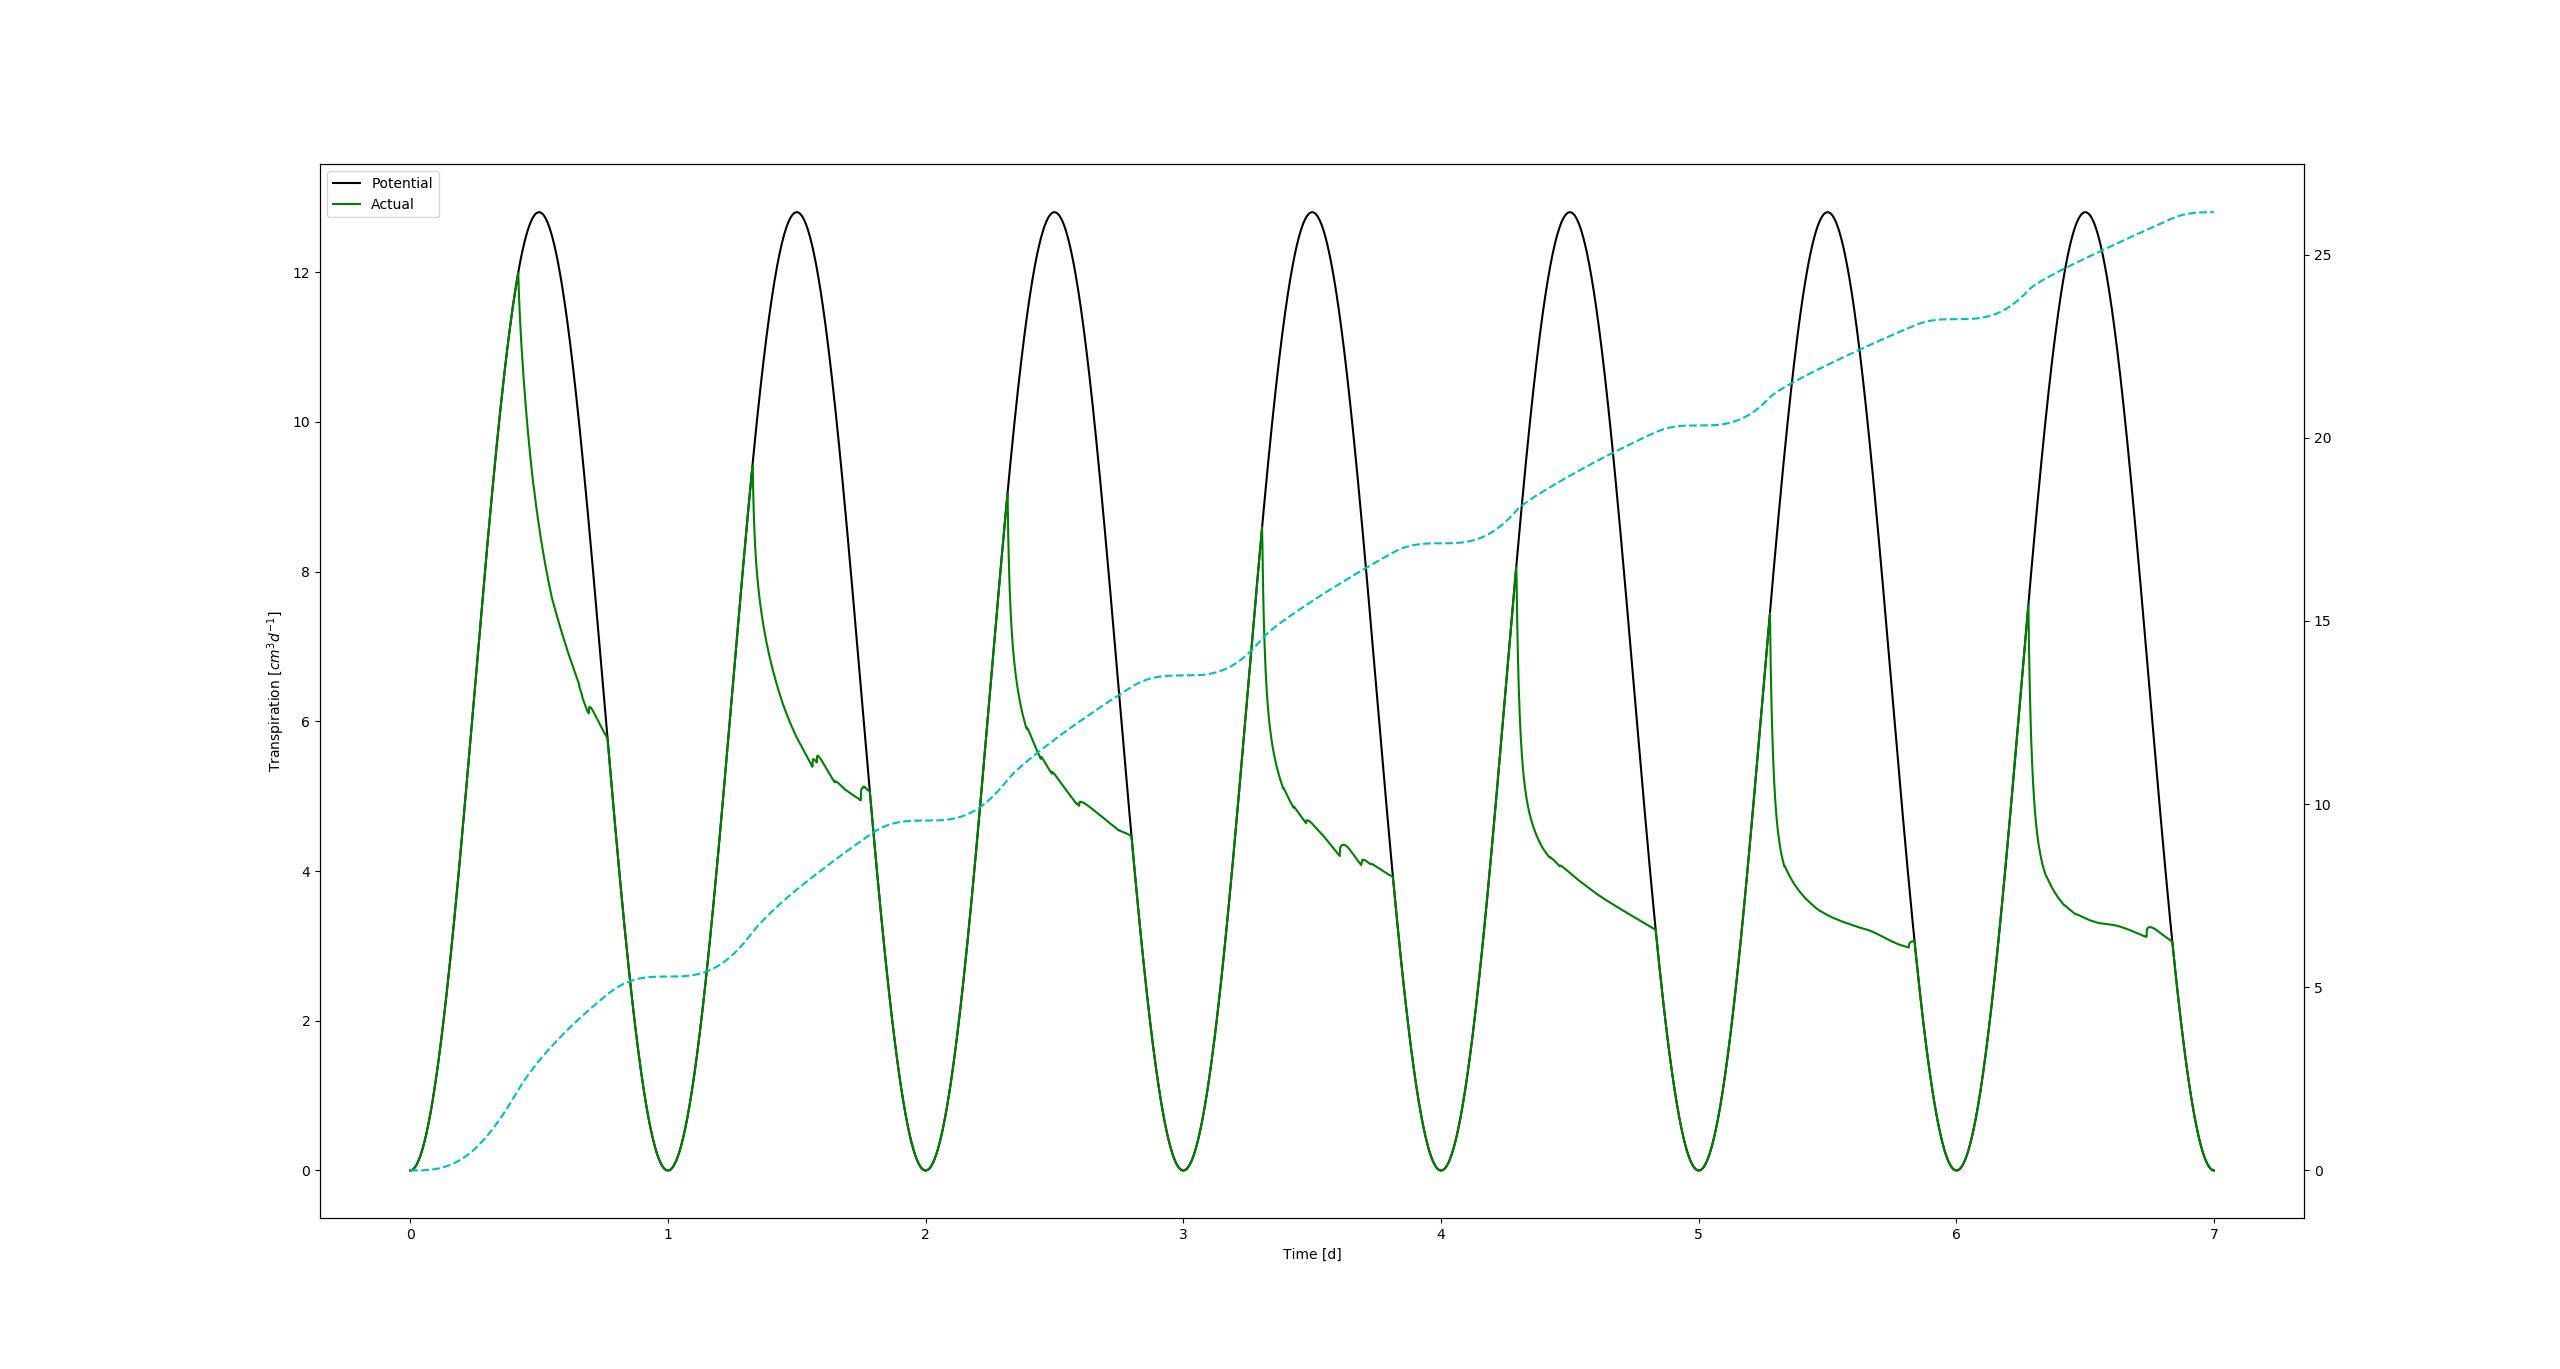
\includegraphics[width=0.99\textwidth]{example7c_no_hydro.png}
\subcaption{Gravi- and Plagiotropism} \label{fig:example7c}
\end{subfigure}
\begin{subfigure}[c]{1\textwidth}
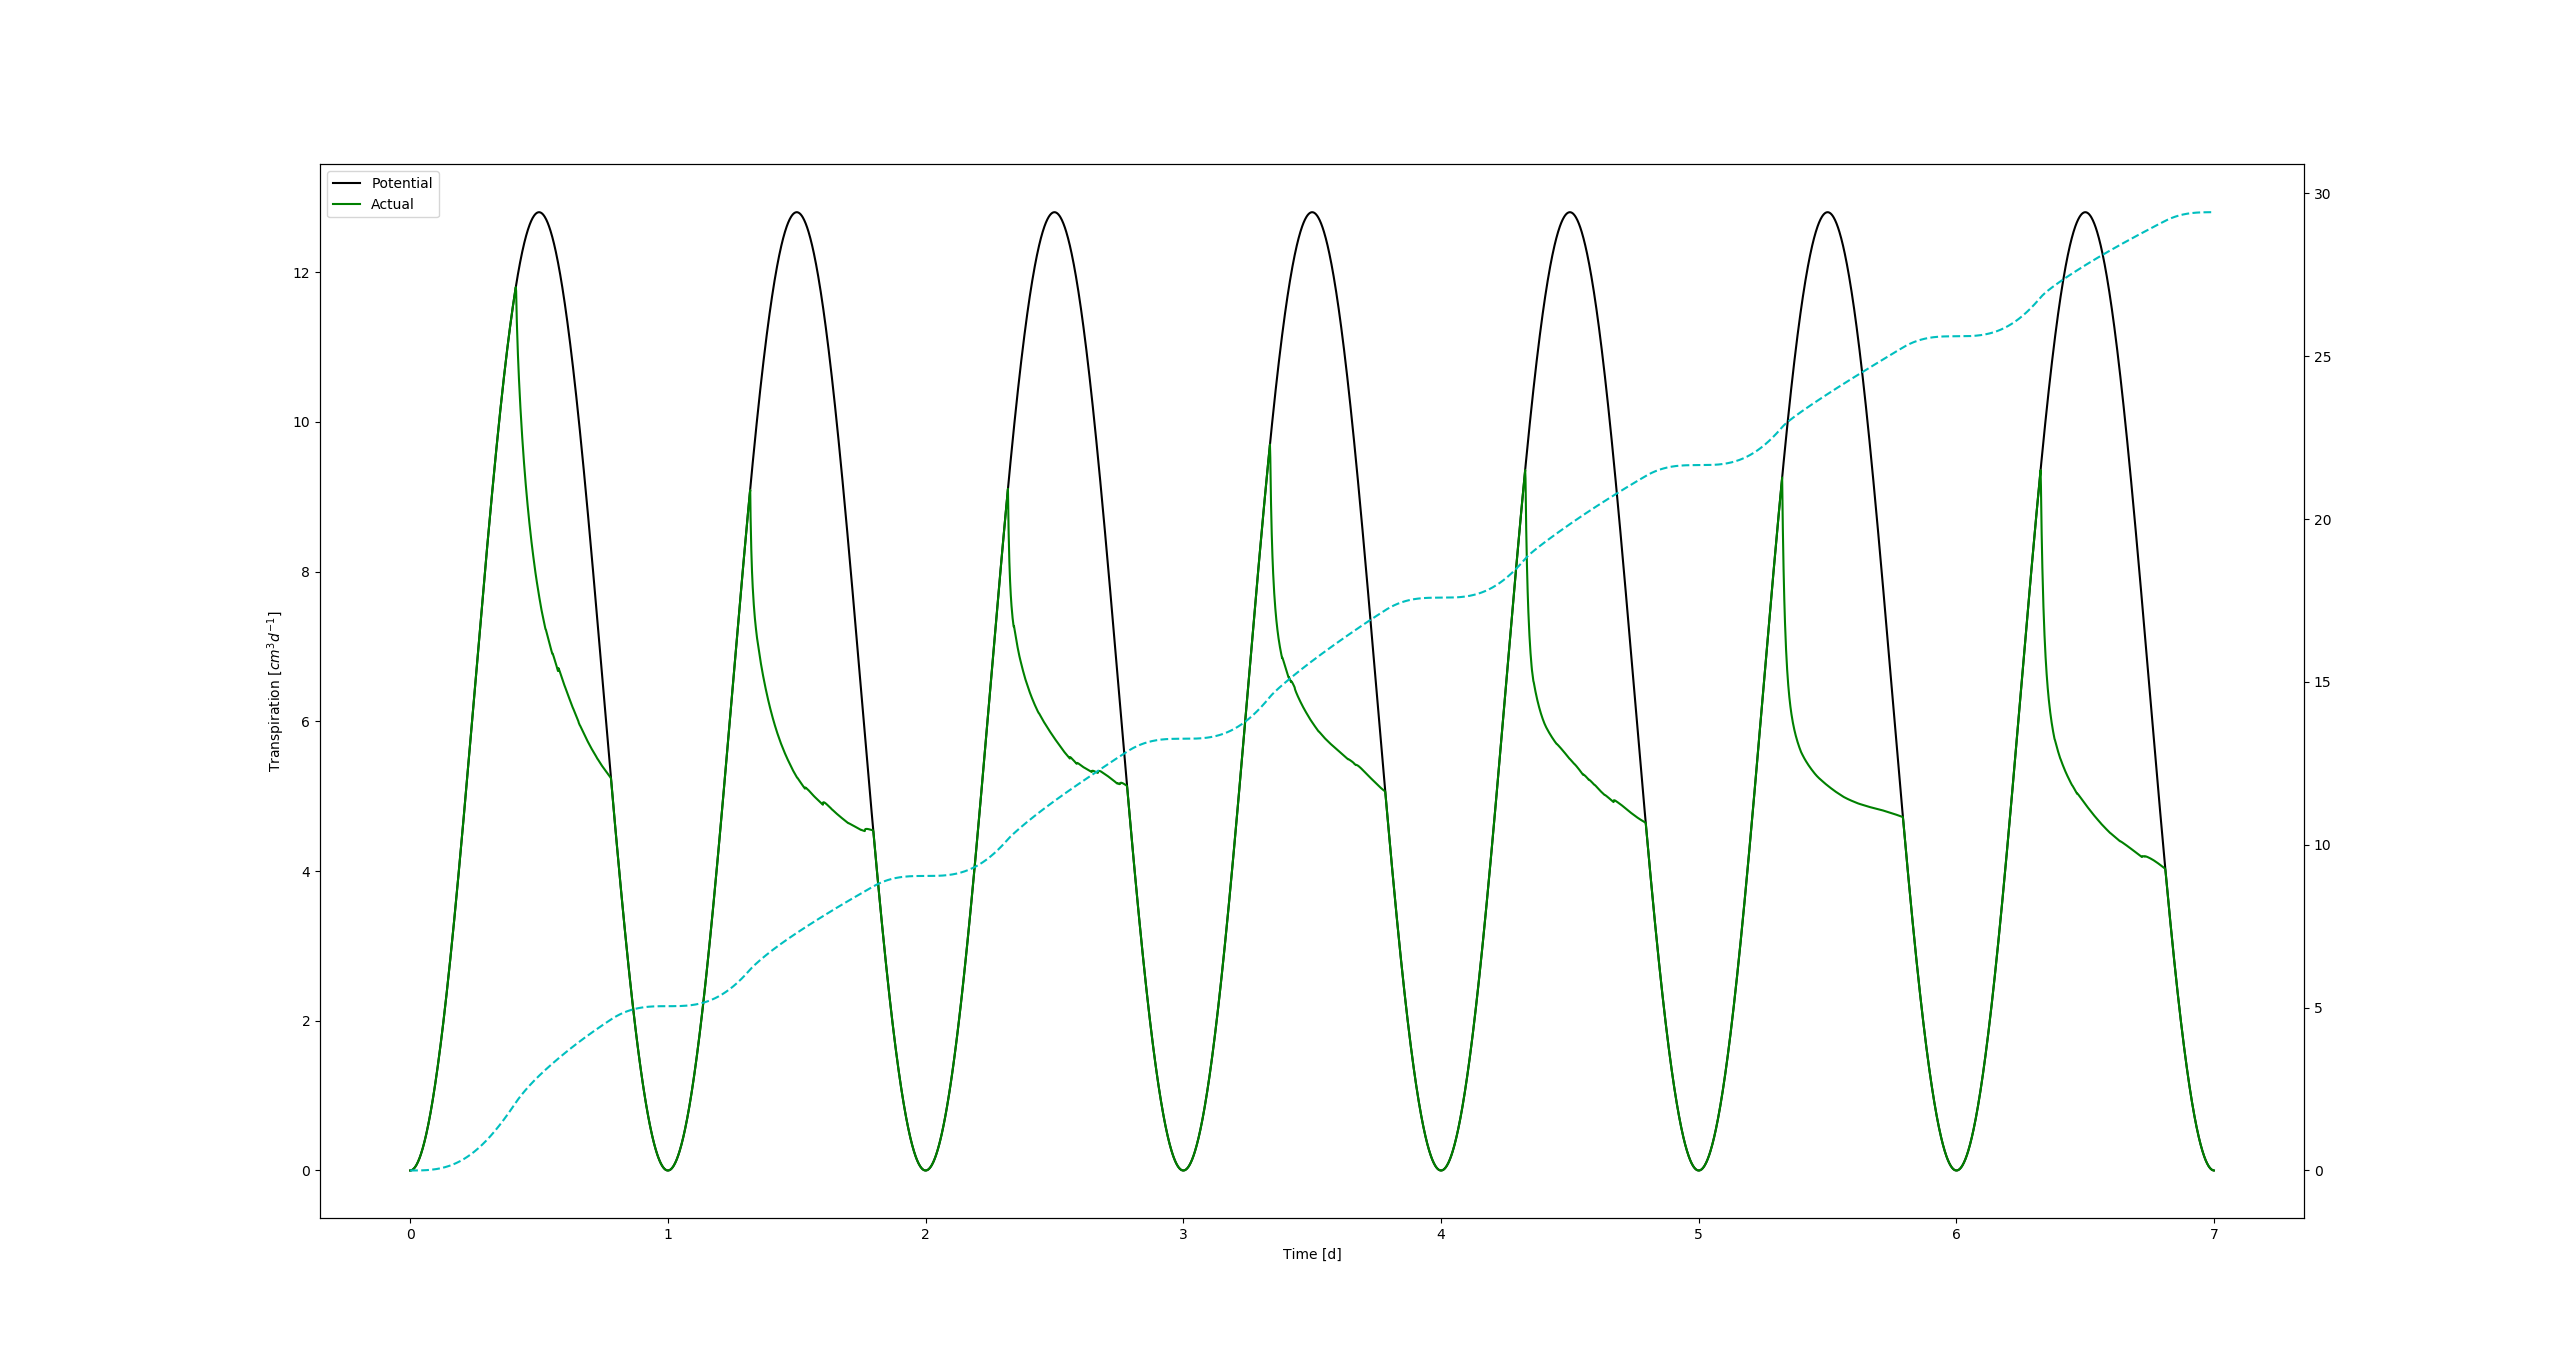
\includegraphics[width=0.99\textwidth]{example7c_simple_hydro.png}
\subcaption{Hydrotropism} \label{fig:example7c_hydro}
\end{subfigure}
\caption{Water uptake a in plant pot} \label{fig:example7c}
\end{figure}

\subsection{Mimicking root growth}
For a pre-grown root architecture, root growth can be mimicked in a dynamic soil-root interactions simulation using the creation times of the root segments. The root axial conductence $k_x$ is set equal to 0 for ``unborne" root segments with negative age. The root radial conductivity, $k_r$ needs to be equal to 0 (not just a small value) for segments with negative  age. 
The parameter \lstinline{initialT} should be equal to 1 if one wants to mimic growth and equal to the final simulation time if not. 
With respect to solute transport, the diffusion coefficient needs to be very small  for unborn segments (?).
